\section{Simulation Experiments}
We implemented our models on network with 3 microgrids. Two of them are operating on solar renewable generation and the other on wind renewable energy. To simulate the renewable generation, we use RAPsim software \cite{rapsim}. RAPsim is an open source simulator for analyzing the power flow in microgrids. It has a provision for simulating the renewable generation, which is the main feature that we use in our experiments. We construct our microgrid model as shown in the Fig 2. We can see that there are three microgrids, two of them operating on the solar energy and the other on the wind energy. The solar microgrid in the right has more capacity than that of the one in the left. These microgrids also have electrical connections from the main grid. Each microgrid provides power to the respective houses on their power line. 


\begin{figure}[thbp] \label{exp}
	\centering
	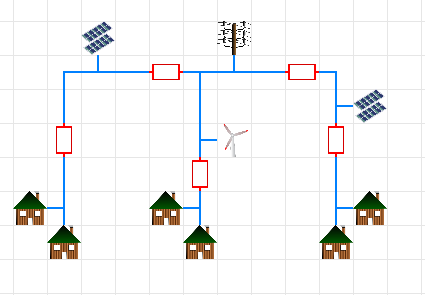
\includegraphics[scale = 0.6]{experimental_setup.jpg}
		\caption{Experimental Setup}
\end{figure}


\subsection{Implementation}

We implement the model we described in the section 2. We call this model as $ADL-sharing$ model. For comparison purposes, we implement following models. 

\begin{itemize}
	\item \textbf{Greedy-ADL model}: In this model, the microgrids will exhibit the greedy behavior. They share the power only if there is excess power after filling up the battery. That is, the action in each instant is bounded by   
	
	\begin{align}
	-min(M, B - nd) \leq max(0,nd - B) 
	\end{align}
	
	That is, if the net demand is negative, decision is taken on amount to power to buy to meet the demand and fill the battery. On the other hand, if the net demand is positive, it is first used to fill the battery and only if there is any excess power left, it will be sold to other microgrids.
	
	\item \textbf{Non-ADL model}:  This model is similar to the $ADL-sharing$ model, but without the integration of ADL demand. In this model, the ADL demand is added to the main demand. Unlike the $ADL-sharing$ model, there is no flexibility of intelligently scheduling the ADL demand. 
	
\end{itemize}

\subsection{Setup}

% \begin{figure}
%still need the trimming of figure. include when we put experimental figures
% 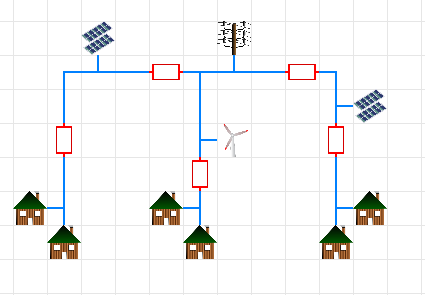
\includegraphics[scale = 0.4]{experimental_setup.jpg}
% \end{figure}

We simulate the above setup for the month of September 2017 and collect the wind and solar renewable power generated each day every hour. The parameters for our experiments are described below. The number of decision time periods is taken to be 4. We consider 3 demand values for all the microgrids - 2, 4 and 6 units. The probability transition matrices for all the 3 microgrids are given below :


\[
P_{1}=
\begin{bmatrix}
0.2 & 0.6 & 0.2 \\
0.1 & 0.2 & 0.7 \\
0.8 & 0.1 & 0.1
\end{bmatrix}
\]

\[
P_{2}=
\begin{bmatrix}
0.2 & 0.2 & 0.6 \\
0.8 & 0.1 & 0.1 \\
0.2 & 0.7 & 0.1
\end{bmatrix}
\]

\[
P_{3}=
\begin{bmatrix}
0.5 & 0.5 & 0 \\
0 & 0.5 & 0.5 \\
1 & 0 & 0
\end{bmatrix}
\]




The price values is considered to be 5, 10 and 15. The Probability transition matrix for the price vector is given below:



\[
Q=
\begin{bmatrix}
0.2 & 0.4 & 0.4 \\
0.1 & 0.5 & 0.4 \\
0.5 & 0.4 & 0.1
\end{bmatrix}
\]


Maximum size of battery and renewable power generated is taken to be 8 units. The maximum power that a microgrid can obtain from the main grid is set to 10 units.

We consider 3 ADLs in our experiment. We assume that all these 3 ADL's are known to microgrids in the first time period. First ADL requires 1 unit of power that needs to be satisfied within the second time period. Second ADL requires 1 unit of power within the third time period. Third ADL requires 2 units of power within the fourth time period.

With this setup, we compare our proposed models. The algorithms are trained for $10^6$ iterations. For comparison purposes, we plot value of threshold $c$ on X-axis and Average reward on Y-axis. Average reward is computed as follows. We run the trained models for 1000 runs and average the reward obtained by each microgrid. 

\subsection{Observations}

\subsection{Discussion}

In Figure 1, we compare our $ADL-sharing$ model with the $Greedy- ADL$. As discussed earlier, in the latter model the sharing of power is done only when there is excess after filling the battery. We can see that the first model outperformed the second model. Even though there will be less buying of power in $Greedy-ADL$, there will be no selling of power as well. Therefore  the overall profit obtained will not be higher than that, when the intelligent decisions are made. Hence we can conclude that the intelligent sharing of power among microgrids yields more profit than that of the non-sharing case. 

In Figure 2, we compare our $ADL-sharing$ model with the $Non-ADL$ model. We can observe from the plot that, our model 1 outperforms the model 3. The reason for that is discussed below. Consider $c \geq 15$, which is the maximum price. In $ADL-sharing$, there is a flexibility to intelligently schedule the ADL activities according to the non-ADL demand and price. But this is not the case with the $Non-ADL$ model. In this case, the penalty will be immediately levied if the demand (including the ADL demand) is not met. This results in the poor performance of $Non-ADL$. Hence we can conclude that intelligently scheduling the ADL demand results in the better performance. 

[update other cases after results]

From the above discussion we can conclude that our proposed algorithm along with the flexible ADL demand integration, is the best algorithm that provides more profits to the microgrids. 